\section{Ablation reporting details}
\label{app:ablations}

The ablation trajectories are shown in Figures~\ref{fig:ablation-half-life} and~\ref{fig:ablation-threshold} in Section~\ref{sec:ablations}.

The ablations use a fixed, accuracy-qualified reference length from aligned RL, shared across configurations. Negative LST indicates responses shorter than this reference; accuracy preservation is evaluated separately on the same fixed easy set.

\begin{table}[htbp]
  \centering
  \caption{\textbf{Ablation endpoint summary at step 1750.}
  Avg.\ Pass@1 is weighted over all 143 evaluation prompts.
  LST is computed against the fixed aligned-RL accuracy-qualified reference.
  The $H=4,\tau=1.0$ run is shared by both comparisons.}
  \label{tab:ablation-endpoints}
  \small
  \resizebox{\linewidth}{!}{%
  \begin{tabular}{ccrrrrr}
    \toprule
    $H$ & $\tau$ & Avg.\ Pass@1 (\%)
    & $\mathrm{LST}_0$ (\%) & $\mathrm{LST}_{100}$ (\%)
    & $\mathrm{LST}_{500}$ (\%) & $\mathrm{LST}_{1000}$ (\%) \\
    \midrule
    2 & 1.00 & 40.14 & 27.79 & 14.64 &  7.29 & 15.49 \\
    4 & 1.00 & 41.85 & 29.20 &  7.63 &  2.01 &  9.06 \\
    8 & 1.00 & 40.49 & 13.01 & 11.00 & -6.21 &  2.91 \\
    4 & 0.85 & 40.91 & 27.55 & 21.24 & 10.84 & 18.42 \\
    4 & 0.75 & 39.31 & 19.15 & 10.97 & -0.68 &  8.11 \\
    \bottomrule
  \end{tabular}%
  }
\end{table}

We compare all five configurations over the shared steps 1--1750.
Table~\ref{tab:ablation-training-diagnostics} reports arithmetic means
of logged per-step scalars; the Pass@1 column instead gives the
unsmoothed evaluation at step 1750. The fresh $H=4,\tau=1.0$ run is
used in both ablations.

\begin{table}[htbp]
  \centering
  \caption{\textbf{LSD training signals in the $H$ and $\tau$ ablations.}
  Sequence and token shares refer to the easy route. Parameter gap is
  the logged maximum absolute teacher--student parameter difference
  before the EMA update. Training statistics average 1750 steps per run.}
  \label{tab:ablation-training-diagnostics}
  \small
  \resizebox{\linewidth}{!}{%
  \begin{tabular}{ccrrrrrr}
    \toprule
    $H$ & $\tau$ & \shortstack{Pass@1\\(\%)}
      & \shortstack{Easy seq.\\(\%)} & \shortstack{Easy tok.\\(\%)}
      & \shortstack{Effective\\OPD coef.}
      & \shortstack{Param. gap\\($\times10^{-5}$)}
      & \shortstack{OPD loss\\($\times10^{-3}$)} \\
    \midrule
    2 & 1.00 & 40.14 & 18.87 & 10.79 & 0.252 & 0.690 & 0.614 \\
    4 & 1.00 & 41.85 & 18.54 & 10.31 & 0.247 & 1.087 & 0.693 \\
    8 & 1.00 & 40.49 & 15.24 &  7.90 & 0.192 & 1.690 & 0.841 \\
    4 & 0.85 & 40.91 & 24.67 & 14.87 & 0.354 & 1.077 & 0.715 \\
    4 & 0.75 & 39.31 & 29.50 & 19.00 & 0.450 & 1.078 & 0.689 \\
    \bottomrule
  \end{tabular}%
  }
\end{table}

\clearpage
\subsection{Teacher lag and distillation exposure}
\label{app:ablation-training-diagnostics}

Increasing $H$ produces a larger teacher parameter lag and a larger
logged SG-FKL loss, while reducing the fraction of tokens sent to OPD.
Thus, the stronger preservation observed for $H=8$ does not require
greater distillation exposure. Instead, the delayed teacher can impose
a stronger constraint on the tokens it supervises. The maximum
parameter gap is a parameter-space diagnostic, not a KL divergence;
its ordering need not match the teacher--rollout log-probability gap.

\begin{figure}[htbp]
  \centering
  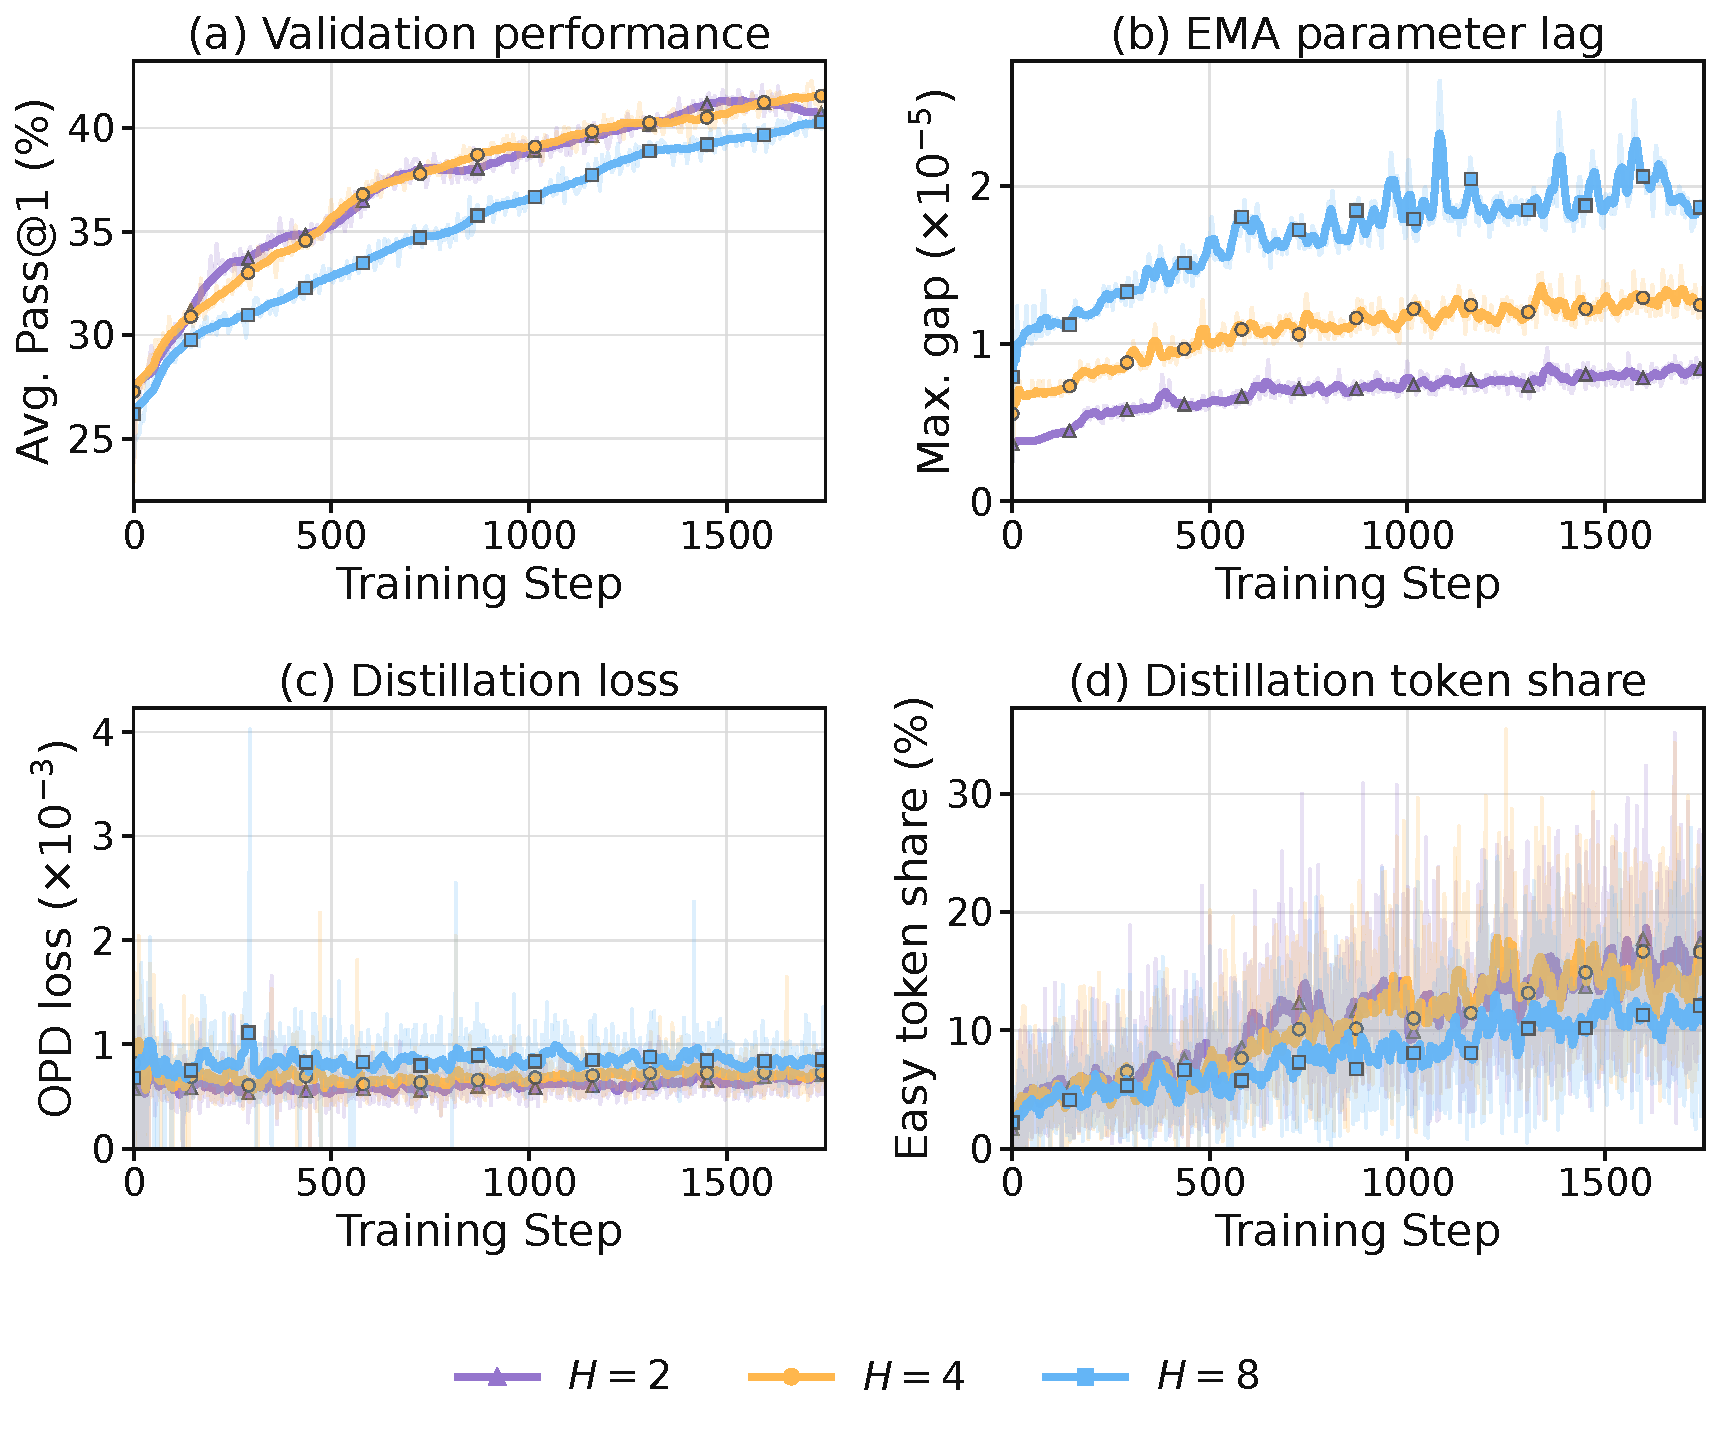
\includegraphics[width=0.90\linewidth]{figures/wandb_half_life_diagnostics.pdf}
  \caption{\textbf{Training signals behind the EMA half-life ablation.}
  All runs use SG-FKL and $\tau=1$.
  Faint lines show raw values; marked curves show centered 21-point
  moving means, using available points at the boundaries.
  Evaluation points are five training steps apart; the other metrics
  are logged every training step.}
  \label{fig:half-life-training-diagnostics}
\end{figure}

\clearpage
\subsection{Routing threshold and preservation pressure}

With eight responses per group, thresholds $\tau=1$, $0.85$, and $0.75$
admit groups with at least eight, seven, and six correct responses,
respectively. Lowering the threshold therefore moves more partially
solved groups to distillation. As shown in
Figure~\ref{fig:threshold-training-diagnostics}, both the easy-route
sequence share and token share increase, along with the logged
effective OPD coefficient. From $\tau=1$ to $0.75$, the mean token
share rises from 10.31\% to 19.00\%, while the effective coefficient
rises from 0.247 to 0.450. The lower Pass@1 at step 1750 is consistent
with more preservation pressure on prompts that still admit incorrect
responses. These coupled changes do not isolate which training signal
causes the performance difference.

\begin{figure}[htbp]
  \centering
  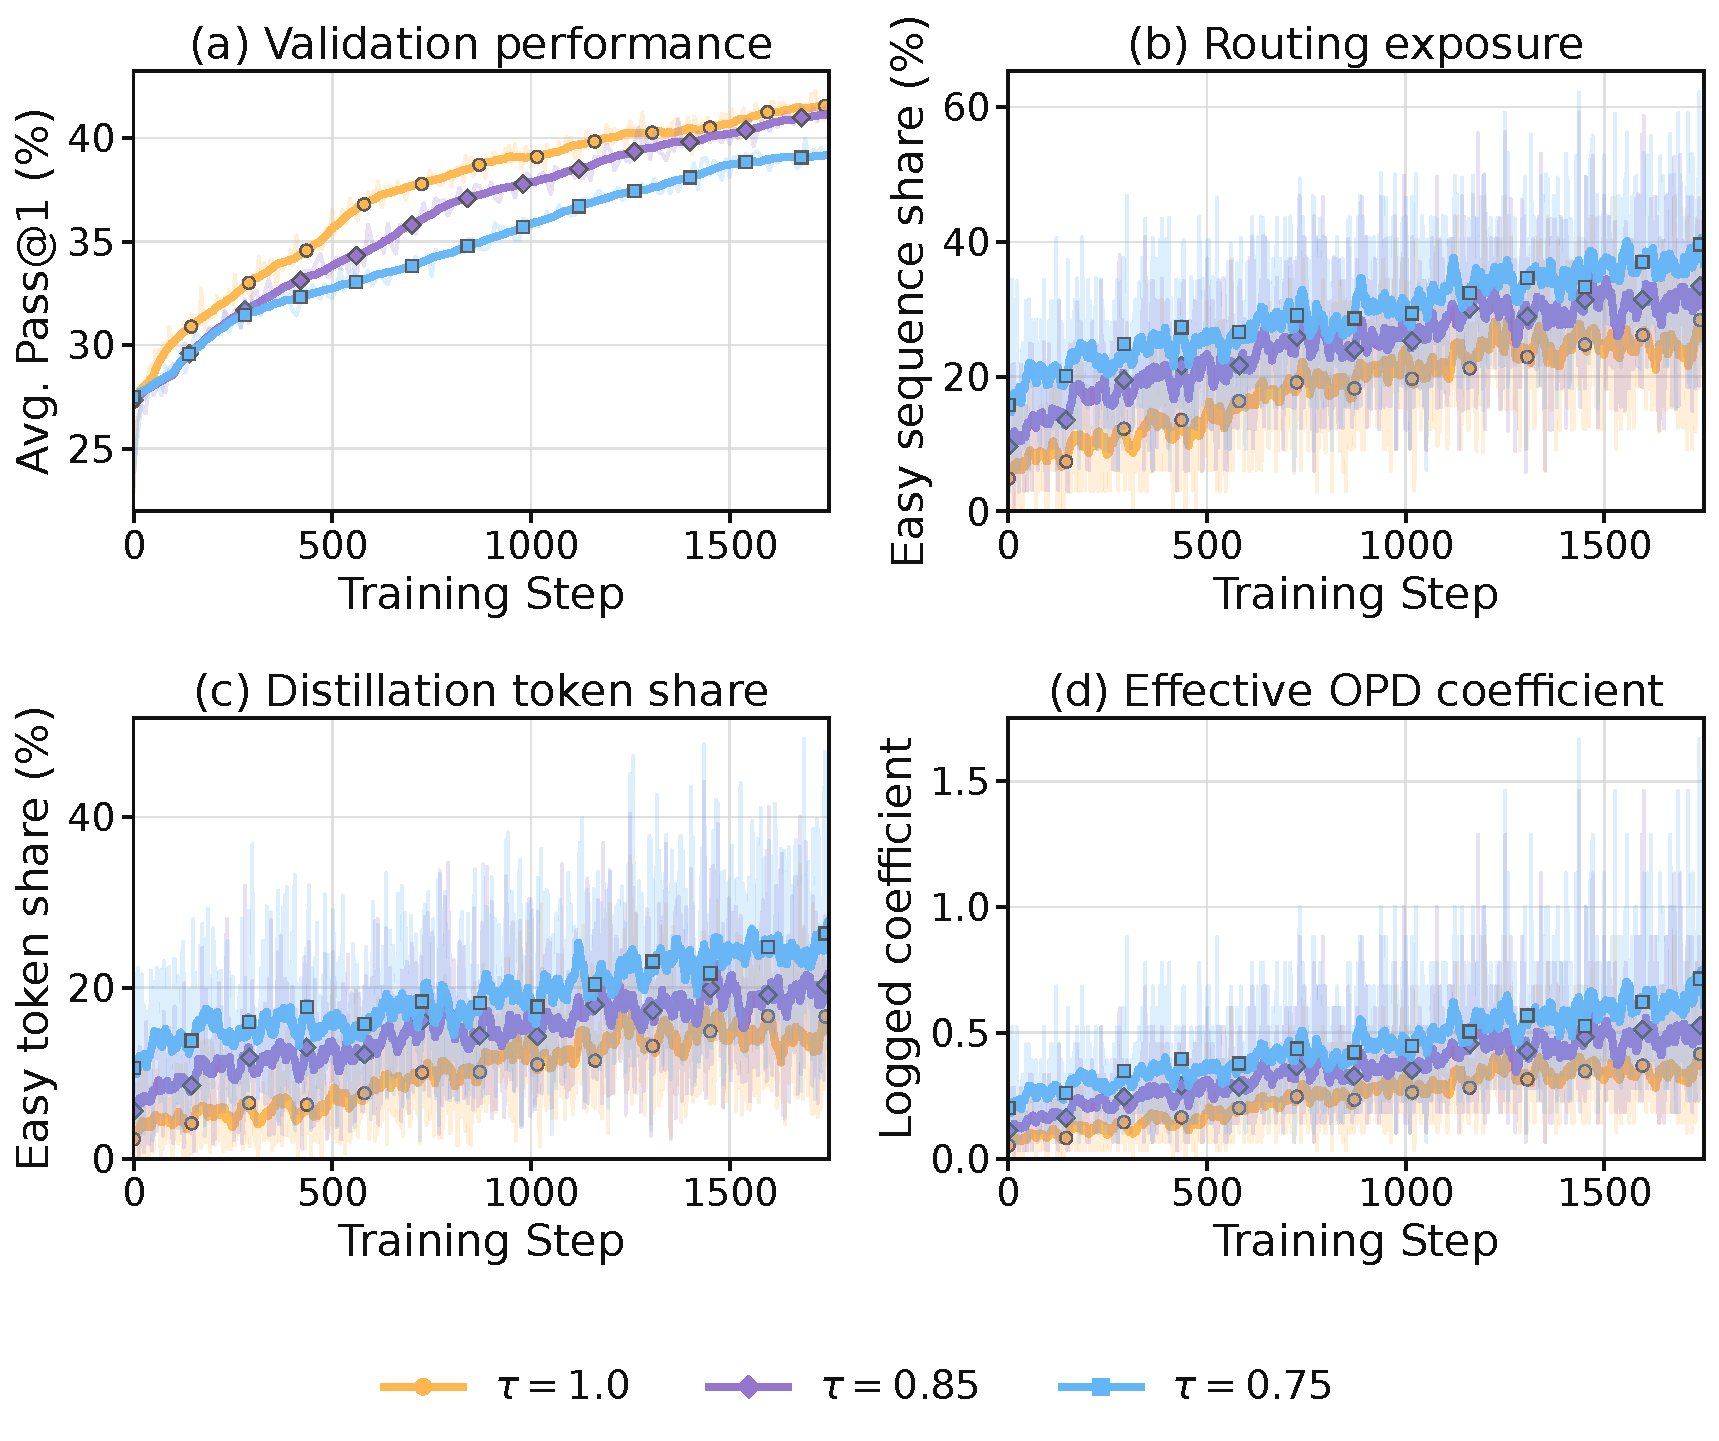
\includegraphics[width=0.90\linewidth]{figures/wandb_threshold_diagnostics.pdf}
  \caption{\textbf{Training signals behind the routing-threshold ablation.}
  All runs use SG-FKL and $H=4$, over steps 1--1750.
  Raw and smoothed curves follow the convention in
  Figure~\ref{fig:half-life-training-diagnostics}.
  Lower thresholds increase the number of sequences and fraction of
  tokens routed to distillation, as well as the effective OPD coefficient.}
  \label{fig:threshold-training-diagnostics}
\end{figure}
